\subsection{MEX 2-1b: Pressure driven percolation, Opalinus claystone}

Participating institutions of MEX 2-1b (see section \ref{sec:mex2-1b}): CAU, UFZ

\begin{table}[ht!]
\caption{MEX 2-1b: Data overview}
\label{tab:dms-mex21b-overview}
\small
\begin{tabular}{l|l|l|l|L{4.7cm}|l}
\hline
\rowcolor{cyan}
Type & Spec. & Owner & Access     & Comment                       & Stat \\ 
\hline
EXP  &       & CAU   & Free       & CAU-Cloud                     & \cellcolor{yellow} \\
\hline \hline
MOD  & LEM   & CAU   & Open       & Executable MATLAB P-file      & \cellcolor{yellow} \\
     &       &       & Free       & Input files will be uploaded  & \cellcolor{yellow} \\
\hline
MOD  & FEM   & UFZ   & Open source & via OpenGeoSys portal        & \cellcolor{yellow} \\
     & VPF   &       & Free       & Input files available         & \cellcolor{green} \\
%
\hline
\end{tabular}
\end{table}
\normalsize

\subsubsection*{CAU (LEM)}

The experimental results of the pressure driven percolation test on the cubic Opalinus claystone samples are uploaded to the IfG (Kiel) NextCloud server. The data is accessible through the following link:\\
\url{https://nextcloud.ifg.uni-kiel.de/index.php/s/EMdNkdF4PRKWCqa}

The experimental data (*.ASCII) of two different stress configurations (section \ref{sec:Percolation_Claystone_Exp}) are uploaded to the server. The data includes the time ($\Delta T=1s$), pump volume ($mL$), given oil pressure ($Bar$) and actual oil pressure in the system ($Bar$). Fig. \ref{fig:Amir_Percolation_Flow_a_Data}
illustrates an example of the plotted borehole pressure vs. flow volume for the $1^{st}$ stress configuration discussed in the section \ref{sec:mex2-1b}.

\begin{figure}[!ht]
\centering
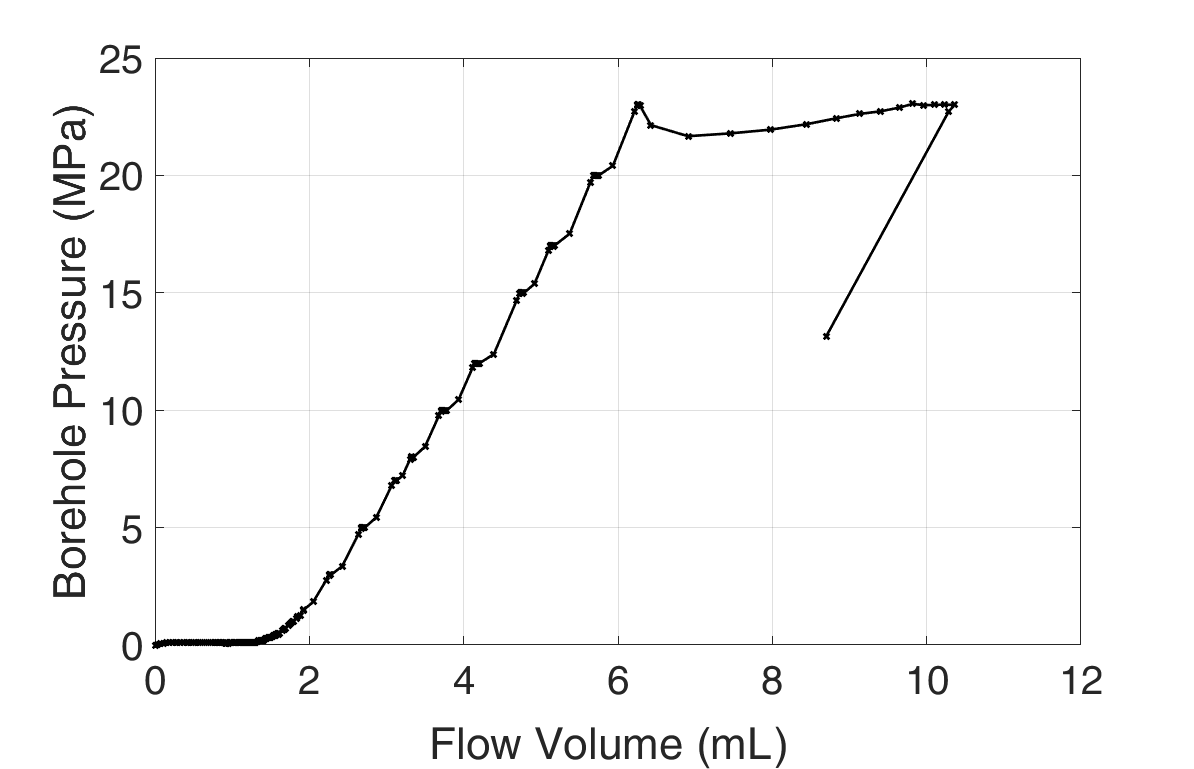
\includegraphics[width=0.85\textwidth]{figures/Amir_Percolation_Flow_a_Data.png}
\caption{The recorded results depicting the evolution of the borehole pressure vs. flow volume for the $1^{st}$ stress configuration}
\label{fig:Amir_Percolation_Flow_a_Data}
\end{figure}

The required LEM code and the input variables of the percolation test on Opalinus claystone samples are uploaded to the IfG (Kiel) NextCloud server. The data is accessible through the following link:\\
\url{https://nextcloud.ifg.uni-kiel.de/index.php/s/tFKKjxnSpgNG25b}

The uploaded protected MATLAB file in a *.p format requires a MATLAB version with a built-in Voronoi Tessellation and Delaunay Triangulation functions. The input variables are prepared in two files for two different stress configurations. Fig. \ref{fig:Amir_ME2_B_Fracture_b_Data}
illustrates an example of the evolved frack surfaces for the $2^{nd}$ stress configuration discussed in the section \ref{sec:mex2-1b}).

\begin{figure}[!ht]
\centering
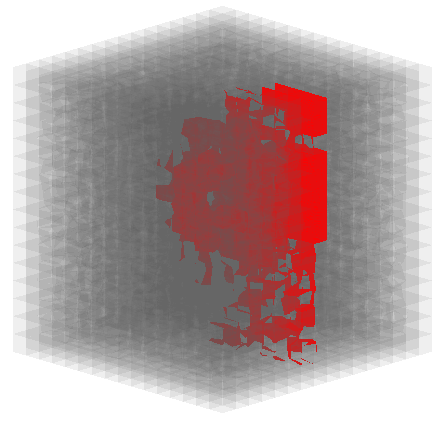
\includegraphics[width=0.75\textwidth]{figures/Amir_ME2_B_Fracture_b_Data.png}
\caption{The frack surfaces (red) for the $2^{nd}$ stress configuration}
\label{fig:Amir_ME2_B_Fracture_b_Data}
\end{figure}

\subsubsection*{UFZ (FEM-VPF)}

MEX 2-1b (UFZ) will be also provided as an OGS benchmark case at:\\
\small
\url{https://www.opengeosys.org/docs/benchmarks/phase-field/phasefield/}
\normalsize

%---------------------------------------------------------
\subsubsection*{Meta Data Overview (according to Dublin Core)}
%---------------------------------------------------------

\begin{table}[!ht]
\caption{MEX 2-1b (CAU)}
\label{tab:dms-mex2-1b}
\small
\begin{tabular}{R{3.5cm}|L{7.5cm}}
\hline
%
Data label & GeomInt, MEX 2-1b, CAU, percolation test, Opalinus clay \\
URL (Experiments) & \url{https://nextcloud.ifg.uni-kiel.de/index.php/s/EMdNkdF4PRKWCqa} \\
URL (Numerics) & \url{https://nextcloud.ifg.uni-kiel.de/index.php/s/tFKKjxnSpgNG25b}  \\
Subject  &  Percolation test (Opalinus claystone)\\
Type of data  & Experimental data, Executable MATLAB P-file, Input parameters\\
Data quality  &  Quality assured data \\
Status of data  &  Unprocessed data\\
Data format  & txt, ASCII, MATLAB executable P-file\\
Creators  &  Kiel University, Institute of Geomechanics and Geotechnics, Ludewig-Meyn-Stra\ss e 10, 24118, Kiel\\
Source/Origin & In-house code \\
Publisher  &  Kiel University, Institute of Geomechanics and Geotechnics, Ludewig-Meyn-Stra\ss e 10, 24118, Kiel \\
Rights holders &  Kiel University, Institute of Geomechanics and Geotechnics, Ludewig-Meyn-Stra\ss e 10, 24118, Kiel \\
Contributors &   Kiel University, Institute of Geomechanics and Geotechnics: Amir Shoarian Sattari, Frank Wuttke\\
Time/period of creation &  2018-2020\\
Language of the content &  English\\
Update policy &  Stored data is final\\
Access permissions & Full access\\
%
\hline
\end{tabular}
\end{table}

\begin{table}[!ht]
\caption{MEX 2-1b (UFZ)}
\label{tab:dms-mex2-1a}
\small
\begin{tabular}{R{3.5cm}|L{7.5cm}}
\hline
%
Data label & GeomInt, MEX 2-1b, UFZ, percolation test, Opalinus clay) \\
URL & \url{https://www.opengeosys.org/docs/benchmarks/phase-field/phasefield/} \\ 
Subject  & Bending fracture test \\
Type of data  & Data set (structured data in a defined format) \\
Data quality  & Quality assured data by benchmarking \\
Status of data  & Processed data \\
Data format  & OGS files \\
Creators  & Yoshioka, Keita  \\
Source/Origin & Open source \\
Publisher  & Helmholtz Centre for Environmental Research UFZ \\
Rights holders & Helmholtz Centre for Environmental Research UFZ \\
Contributors & Yoshioka, Keita \\
Time/period of creation & 2019-2020 \\
Language of content & English \\
Update policy & To be merged to OGS benchmarks (see below) \\
Access permissions & Free access \\
%
\hline
\end{tabular}
\end{table}
